\documentclass[../main/main.tex]{subfiles}
\begin{document}



\chapter{The Path integral in Quantum Mechanics}

Path Integral will be the main tool we will use in this course in order to study QFT.
We will start introducing this tool in special case of Quantum Mechanics.

\section{Intuitive Introduction to Path Integrals}
\textsf{Rattazzi~\cite{Rattazzi:2011aa} sec. 1.1.1 - 1.1.3}\\

One of the important experiments that show the fundamental difference between Quantum and Classical Mechanics is the double slit experiment. It is interesting with respect to the path integral formalism because it leads to a conceputal motivation for introducing it.

Consider a source $S$ of approximatively mono-energetic particles, electrons for instance, placed at position $(x_i,y_i)$. The flux of electrons is measured on a screen facing the source. Imagine now placing a third screen in between the ohers, with two slits on it, which can be opened or closed. When the first is open and the second closed we measure the flux $F_1$, when the first slit is closed and the second open we measure a flux $F_2$ and when both slits are open we measure the flux $F$.

One finds in general $F=F_1+F_2+F_{int}$, and the structure of $F_{int}$ precisely corresponds to the interference between two waves passing respectively through 1 and 2:
\[F=|\phi_1+\phi_2|^2=\underbrace{|\phi_1|^2}_{F_1}+\underbrace{|\phi_2|^2}_{F_2}+\underbrace{\phi_1\phi_2^*+\phi_2\phi_1^*}_{F_{int}}\]
where $\phi_i$ is the probability amplitude for a point-like particle position and $\vert\phi_i\vert^2$ the corresponding probability density.

The idea behind the path integral approach to QM is to take the implications of the double slit experiment to its extreme consequences. One can immagine adding extra screens and drilling more and more holes through them, generalising the result of the double slit experiment by the superposition principle.

Let's denote as follows the superposition of N slits fluxes:
\[\Phi={\sum_{i=1}^N}\,\phi(y^i_A)\]
where $\phi(y^i_A)$ denotes the flux of the particle whose trajectory goes through the $i$-th slit positioned in the coordinate $y^i_A$ of the screen placed in $x_A$.
Nothing stops us from taking the ideal limit where $N\to\infty$ and the holes fill all the surface. The sum $\sum_i$ becomes now an integral over $y_A$:
\[\Phi=\int\de y_A\phi(y_A)\]

We can go on and further refine our trajectories by adding more and more screens between the source and the final screen. In the limit in which the added screens become infinitesimally close, we have specified all possible paths $y(x)$:
\[\Phi=\int\de x\int \de y_x\phi(y(x))\]
where $\phi(y(x))$ is the flux corresponding to the path $y(x)$. 

\begin{figure}[H]
\centering
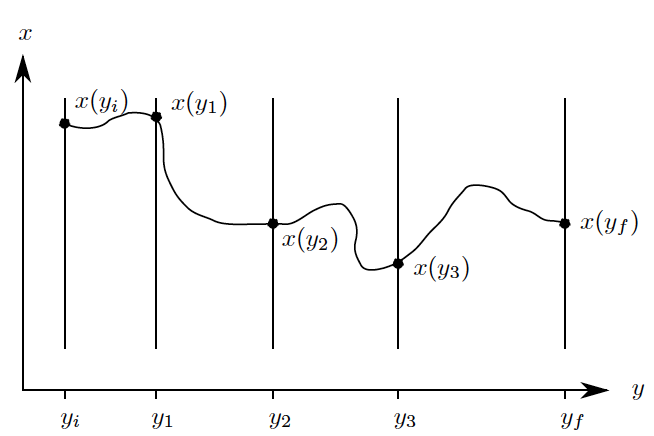
\includegraphics[width=7cm]{../img/Path-int-slit.png}
\caption{$y_i$ denotes position of screens, while $x(y_i)$ are the positions where the particle is found in each screen. Notice that the role of $x$ and $y$ are inverted respect to our notation.}
\end{figure}

We then arrived at a formal representation of the probability amplitude as a sum over all possible trajectories:
\begin{equation}\label{eqn:sketch-total-phase-trajectory}
\Phi=\sum_{\substack{\text{All trajectories}\\\{x(t),y(t)\}}}\phi(\{x\})
\end{equation}

How do I make sense of this? What $\Phi$ is and how do I make sense of this sum?
Moreover, I'd like that for $\hbar\to0$ I should go back to Classical Mechanics.\footnote{See Rattazzi and MacKenzie chap. 3.} This implies that $\phi$ must depends on $\hbar$ in someway.
Since $\hbar$ has dimensionality [Energy]$\times$[Time], one can guess that 
\begin{equation}\label{eqn:path-exp-formula}
\phi(\gamma)=e^{i\frac{S[\gamma]}{\hbar}}
\end{equation}
where $S$ is the action which describes the classical trajectories via the principle of least action. This means that we associate to each trajectory $\gamma$ a phase related to the action $S[\gamma]$. Recall that the classical trajectories are given by the stationary points of $S[\gamma]$ ($\delta S[\gamma]=0$).
 
Let's analyze our guess. The choice $\phi(\gamma)=f(S[\gamma]/\hbar)$ is natural, since in this way the argument is adimensional. The choice of the exponential function seems promising for two reasons:

\begin{enumerate}
\item The requirement $\delta S[\gamma]=0$ for $\hbar\to0$ is heuristically seen to hold. In a macroscopic, classical, situation the gradient $\delta S/\delta\gamma$ is for most trajectories much greater than $\hbar$. Around such trajectories the phase $e^{iS/\hbar}$ oscillates extremely rapidly and the sum over neighbouring trajectories will tend to cancel. 

On the other hand, on a classical trajectory $\gamma_{cl}$ the action $S$ is stationary. Therefore in the neighbourhood of $\gamma_{cl}$, $S$ varies very little, so that all trajectories in a tube centred around $\gamma_{cl}$ add up coherently in the sum over trajectories. 

Indeed, this means that in the exact limit $\hbar\to0$ these effects becomes dramatic and only the classical trajectory survives.

\item Eq. \eqref{eqn:path-exp-formula} leads to crucial composition property. Indeed the action for a path $\gamma_{12}$ obtained by joining two subsequent paths $\gamma_1$ and $\gamma_2$ satisfies the simple additive relation
\[S[\gamma_{12}]=S[\gamma_1]+S[\gamma_2]\]
Thanks to eq.\eqref{eqn:path-exp-formula} the additivity of $S$ translates into a factorization property for the amplitude:
\[\phi[\gamma_{12}]=\phi[\gamma_1]\phi[\gamma_2]\]
This feature is required for our theory, as it describes composition of paths and the corresponding probability.

\end{enumerate}


\section{From Schroedinger Equation to the Path Integral}
\textsf{Rattazzi~\cite{Rattazzi:2011aa}, sec. 1.1.4; Sredniki~\cite{Srednicki:2007aa} chap. 6; Peskin~\cite{Peskin:1995aa} chap. 9.1; MacKenzie~\cite{MacKenzie:2000aa} sec. 2.1, 2.2.1}\\

In the previous discussion gave us the idea behind Path Integrals formulation in QM, now we will derive it more formally starting from Schrödinger equation. 

The transition amplitude for a particle in QM reads

\[\braket{x_f(t_f)}{x_i(t_i)}=\bra{x_f}e^{-i\frac{\hat H}{\hbar}(t_f-t_i)}\ket{x_i}\]
In order to evaluate this quantity we split $t_f-t_i$ in $N$ pieces with $N$ large. Let $\delta t=(t_f-t_i)/N$. Recall that $\int\de x\ket{x}\bra{x}=1=\int\de p\ket{p}\bra{p}$. Then
\begin{align}\label{eqn:intro-Path-Int-deco}
\braket{x_f(t_f)}{x_i(t_i)}=\int\p{\prod_{j=1}^{N-1}\de x_j}
&\bra{x_f}e^{-i\frac{\hat H}{\hbar}\delta t}\ket{x_{N-1}}
\bra{x_{N-1}}e^{-i\frac{\hat H}{\hbar}\delta t}\ket{x_{N-2}}
\dots
\bra{x_2}e^{-i\frac{\hat H}{\hbar}\delta t}\ket{x_1}
\bra{x_1}e^{-i\frac{\hat H}{\hbar}\delta t}\ket{x_i}
\end{align}
For each piece we have
\begin{equation}\label{eqn:intro-path-int-integ-p}
\bra{x'}e^{-i\frac{\hat H}{\hbar}\delta t}\ket{x}=\int\de p\braket{x'}{p}\bra{p}e^{-i\frac{\hat H}{\hbar}\delta t}\ket{x}
\end{equation}
If we stick to the simply case $\hat H=\hat p/2m+V(\hat x)$ where we denote the kinetic operator as $T(\hat p)=-i\frac{\hat p^2}{2m\hbar}\delta t$ and the potential $U(\hat x)=-iV(\hat x)\delta t/\hbar$, we can write
\begin{align*}
\bra{p}\exp{T(\hat p)+U(\hat x)}\ket{x}
=\bra{p}e^{T(\hat p)}e^{-T(\hat p)}e^{T(\hat p)+U(\hat x)}e^{-U(\hat x)}e^{U(\hat x)}\ket{x}=e^{T(p)}e^{U(x)}\bra{p}e^{C(\hat p,\hat x)}\ket{x}
\end{align*}
where
\[e^{C(\hat p,\hat x)}=e^{-T(\hat p)}e^{T(\hat p)+U(\hat x)}e^{-U(\hat x)}\]
The operator $C$ is given, using Baker-Campbell-Hausdorff formula
\footnote{Let $e^Xe^Y=e^Z$ for some operators X,Y,Z, then \[Z(X,Y)=\log(\exp X\exp Y)= X + Y + \frac{1}{2}[X,Y] + \frac{1}{12}\left ([X,[X,Y]] +[Y,[Y,X]]\right )- \frac {1}{24}[Y,[X,[X,Y]]]+\dots\]}
 twice, as a series of commutators between $T$ and $U$
\begin{align*}
C=\frac12[T,U]+\frac{1}6([T,[T,U]]+[U,[U,T]])+...
\end{align*}
If all commutators in the expression of $C$ are $O(1)$, then all the terms of the expansion of $C$ are $O((\delta t)^2)$ and therefore can be neglected. However, this assumption is not immediate, for example $[\hat p,V(\hat x)]=-iV'(\hat x)$ implies that in order to neglect $C$ all derivatives of $V$ must be bounded. Then, if the derivatives of $V$ are bounded, the contribution of the operator $\hat x$ in the expansion of $C$ is a bounded contribution and in the limit $\delta t\to0$ vanishes. \\
The only remaining potential problem to concentrate on the $\delta t\to0$ limit is represented by the integration over powers of $p$ in \eqref{eqn:intro-path-int-integ-p}. Indeed what we are integrating is a function that goes approximatively as the gaussian $\exp(-\delta t\,p^2)$, therefore the leading contribution to the $p$ integral is the one with $p\sim\delta t^{-1/2}$, showing that $p$ diverges in the small $\delta t$ limit. Nevertheless one can actually prove\footnote{See Rattazzi pag 14 for details.} that for small $\delta t$:
\[\bra{p}e^{C(\hat p,\hat x)}\ket{x}\simeq\braket{p}{x}(1+O(\delta t^{3/2}))\]
and even if I consider all $N=1/\delta t$ contributions of the form $\bra{p}e^{C(\hat p,\hat x)}\ket{x}$ in \eqref{eqn:intro-Path-Int-deco}, they can be neglected, since the final result is convergent to 1: 
\[\lim_{\delta t\to0}(1+a\,\delta t^{3/2})^{1/\delta t}=1\]
Therefore we can reasonably neglect contributions of $C$ and then
\[\lim_{\delta t\to0}\bra{x'}e^{-i\frac{\hat H}{\hbar}\delta t}\ket{x}
\simeq\lim_{\delta t\to0}\int\de p\exp{-i\frac{\delta t}{\hbar}\left[\frac{p^2}{2m}+V(x)\right]}\cdot\underbrace{\frac{\exp{i p(x'-x)/\hbar}}{2\pi\hbar}}_{\braket*{x'}{p}\braket{p}{x}}\]
Now we introduce the variable $\dot x=(x'-x)/\delta t$: 
\[\lim_{\delta t\to0}\bra{x'}e^{-i\frac{\hat H}{\hbar}\delta t}\ket{x}
=\lim_{\delta t\to0}\int\frac{\de p}{2\pi\hbar}\exp{-i\frac{\delta t}{\hbar}\p{\frac{p^2}{2m}+V(x)-p\dot x}}\]
and performing the change of variable $p'=p-m\dot x$ we obtain
\begin{align*}
\lim_{\delta t\to0}\bra{x'}e^{-i\frac{\hat H}{\hbar}\delta t}\ket{x}
&=\lim_{\delta t\to0}\int\frac{\de p'}{2\pi\hbar}\exp\bigg\{-i\frac{\delta t}{\hbar}\bigg(\frac{p'^2}{2m}+\underbrace{V(x)-\frac12m\dot x^2}_{-\mathcal L}\bigg)\bigg\}\\
&=\lim_{\delta t\to0}\underbrace{\sqrt{\frac{m}{2\pi i\hbar\,\delta t}}}_{\kappa}\exp{i\frac{\delta t}{\hbar}\mathcal L(x,\dot x)}
\end{align*}
where we introduced the factor $\kappa$ (that depends on $\delta t$) in order to simplify the notation. When I introduce this into eq.~\eqref{eqn:intro-Path-Int-deco} we have the following formula for the transition amplitude ($x_0=x_i$, $x_N=x_f$):

\begin{align*}
\braket{x_f(t_f)}{x_i(t_i)}
&=\lim_{\delta t\to0}\int\prod_{j=1}^{N-1}\de x_j
\kappa^N\exp{\frac{i}{\hbar}\sum_{m=0}^{N-1}\delta t\,\mathcal L(x_m,\dot x_m)}\\
&=\lim_{\delta t\to0}\kappa\int\prod_{j=1}^{N-1}(\de x_j\, \kappa)\exp{\frac{i}{\hbar}S(x_f,x_i)}
\end{align*}
We define the following functional measure over the space of trajectories\footnote{For the moment is not  clear if this functional is well defined and is a measure, this is just an anticipation of following results.}:
\begin{equation}\boxed{
\int_{C_T[x_i,x_f]} \mathcal Dx = \lim_{\delta t\to0} \kappa \int\prod_{j=1}^{N-1}(\de x_j\,\kappa)
}\end{equation}
Here $C_T[x_i,x_f]$ are all possible configurations on $x$ that start in $x_i$ and end in $x_f$ over a time $T=t_f-t_i$, i.e. is the set of all possible path $x(t)$ such that $x(t_i)=x_i$ and $x(t_i+T)=x(t_f)=x_f$. We call ${C_T[x_i,x_f]}$ \textbf{space of configurations}. The weight $\exp{\frac{i}{\hbar}S(x_f,x_i)}$ is the phase related to eq.\eqref{eqn:path-exp-formula}. Therefore I obtain
\begin{equation}\label{eqn:transition-measure-config}\boxed{
\braket{x_f(t_f)}{x_i(t_i)}=\int_{C_T[x_i,x_f]} \mathcal Dx\,\exp{\frac{i}{\hbar}S(x_f,x_i)}
}\end{equation}
This is just the analogous of eq.\eqref{eqn:sketch-total-phase-trajectory}. Notice that eq.\eqref{eqn:transition-measure-config} is manifestly invariant under the symmetries of our theory. 

The construction we made has no rigor, but clarify the idea behind Path Integrals theory. The result we obtained so far is the replacement of the sum into eq.\eqref{eqn:sketch-total-phase-trajectory} with an integral, hoping in a convergent expression. This is not obvious, indeed this does not happen in general. 

This definition has some problematic points, that sometimes does not matter and one can skip on them in a straightforward way, but can also became crucial in order to obtain the results we obtained in operatorial approach. For example we assumed that trajectories were smooth and we can differentiate them, but this is not going to be true. Quite the opposite, the fact that trajectories may not be smooth leads to the contact between Path Integral approach and operatorial formalism of QM. 

We won't examinate details of mathematical structure of functional formalism behind Path Integrals since it is not really interesting from the physical point of view, rather we focus on problematical aspects and special features of this formalism in order to obtain a deeper understanding of the physics. 

Before proceeding with technical developments, it is worth assessing the role of the path integral in quantum mechanics. As it was hopefully highlighted so far, the path integral formulation is conceptually advantageous over the standard operatorial formulation of QM, in that the ``good old'' particle trajectories retain same role. The P.I. is however technically more involved. When working on simple quantum systems like the hydrogen atom, no technical profit is really given by path integrals. Nonetheless, after overcoming a few technical difficulties, the path integral offers a much more direct viewpoint on the semiclassical limit. Similarly, for issues involving topology (like the origin of Bose and Fermi statistics, the Aharonov-Bohm effect, charge quantization in the presence of a magnetic monopole, etc$\dots$) path integrals offer a much better viewpoint. Finally, for advanced issues like the quantization of gauge theories and for effects like instantons in quantum field theory it would be hard to think how to proceed without path integrals.

\section{The Partition Function}
\textsf{Skinner~\cite{Skinner:2018aa} chap. 1}\\

We want to generalize results of the previous section. 
What we have done, is to sum over all possible configurations of the field with a certain measure and weight them with a weight function that is essentially the action:
\begin{equation}\label{eqn:dfn-partition-function}\boxed{
\mathcal Z(\lambda, m,\dots)=\int_{\phi\in C}\mathcal  D\phi\,\exp{\frac i\hbar S[\phi]}
}\end{equation}
This is the generic form for a \textbf{path integral} and in particular is the \textbf{partition function} for a certain theory. In order to describe the theory we have to specify:
\begin{enumerate}
\item $M$: The manifold where out QFT theory lives, in particular we have to specify its dimension $d$ and, if it exists, the space's metric $g$ (we can also think about a metric with some degree of freedom, such in Quantum Gravity).
\item $\phi$: Fields over the space, that are generically maps from $M$ to some target space (e.g. $\RR$, $\CC$, vector fields, gauge group, gauge bundle, etc.)
\item $C$: Space of allowed field configurations (possibly with some boundary conditions)
\item $\lambda$: Other parameters of the theory (such as mass $m$ etc.)
\item $\mathcal L$: The Lagrangian of our theory
\item $S$: The action (depends on all the other parameters)
\[S[\phi]=\int_M\de^dx\sqrt{|g|}\mathcal L(\phi, \partial \phi, \lambda, m, \dots)\]
\item$\mathcal D\phi$: the measure of integration
\end{enumerate}
%
Once I have specified this items i can obtain a well defined partition function form my theory eq.\eqref{eqn:dfn-partition-function}. Moreover starting with partition function we can compute correlation functions.
On the other hand partition function can depends on other parameters $\lambda'$ to which the action is independent. Notice that  eq.\eqref{eqn:dfn-partition-function} can be also a divergent, but this happens often and doesn't really matter. The important aspect is how the behaviour of the partition function depends on its parameters. 

The name ``partition function'' comes from statistical mechanics\footnote{See also MacKenzie~\cite{MacKenzie:2000aa} chap. 5, Zinn-Justin~\cite{Zinn-Justin:2002aa} sec. 2.4 and Nakahara~\cite{Nakahara:2003aa} sec. 1.3.1, 1.3.2 for a furthered description of this correspondence between path integral formulation and partition functions in statistical mechanics.}: consider for instance a map from the circle to another target space
\[x:S^1\to N\qquad x(0)=x(T)=y\in N\]
When we go to the Euclidian space by sending\footnote{Notice that parametrizing $S^1$ into the Euclidian, we introduced an additional factor $i$, that multiplied by the factor $i$ present in the definition of partition function gives a minus. This will happen often when we compute partition integrals explicitly.} $t\to i\tau$ ($\hbar =1$) and we compute the path integral for some boundaries condition we obtain (notice that initial and final positions are the same)
\[\int_{x\in C_T[y,y]}\mathcal Dx \,e^{-S[x]}=\bra{y}e^{-HT}\ket {y}\]
and this is related to partition function of statistical mechanics, since this means that calculating the statistical partition function by tracing over all the Hilbert space $\mathcal H$
\[\Tr_{\mathcal H}(e^{-HT})=\int \de y\bra{y}e^{-HT}\ket{y}=\int\de y\int_{x\in C_T[y,y]}\mathcal D xe^{-S[x]}\]
is the same as taking path integral without boundaries, i.e. integrating over all possible configurations $y\in S^1$. 
\[\Tr_{\mathcal H}(e^{-HT})=\int_{x\in C_{S1}}\mathcal Dxe^{-S[x]}\]


\section{Operators and Time Ordering}
\textsf{Rattazzi~\cite{Rattazzi:2011aa} sec. 1.4, Skinner~\cite{Skinner:2018aa} sec. 1.2, 3.1; MacKenzie~\cite{MacKenzie:2000aa} chap. 6, 7; Zinn-Justin~\cite{Zinn-Justin:2002aa} sec. 2.4.2}\\

Now we want to see how to use path integral in order to compute operator matrix elements and more in general correlation functions. Notice that this problem depends on which picture (Heisenberg or Schrödinger) we use. In the Heisenberg picture operators evolve with time according to
\[\hat O(t)=e^{\frac{i\hat Ht}{\hbar}}\hat Oe^{\frac{-i\hat Ht}{\hbar}}\]
where $\hat O$ is the time independent operator in the Schröedinger picture, while states are time independent. In Schröedinger picture operators are time independent, while states evolves according to
\[\ket t=e^{\frac{i\hat Ht}{\hbar}}\ket{t=0}\]
For instance if we want to compute the value of position $\hat x$ on a state for a given time $t$ we see that
\[\hat x(t)\ket{x,t}=e^{\frac{i\hat Ht}{\hbar}}\hat xe^{-\frac{i\hat Ht}{\hbar}}e^{\frac{i\hat Ht}{\hbar}}\ket{x, t=0}=xe^{\frac{i\hat Ht}{\hbar}}\ket{x, t=0}=x\ket{x,t}\]
We want to prove that matrix elements of \emph{local} operators\footnote{Local operators are operators that depend on the value of the field (and perhaps finitely many derivatives) at a single point in $M$.} can be computed using path integrals using the following formula
\begin{equation}\boxed{
\int_{C_{t_f-t_i}[x_i,x_f]}\mathcal Dx\,O(x(t))\exp{\frac i\hbar S[x]}=\bra{x_f,t_f}\hat O(\hat x(t))\ket{x_i,t_i}
}\end{equation}
Therefore we have to relate matrix elements with the expression eq.~\eqref{eqn:transition-measure-config}. In order to do that I have to find a way to remove $\hat O(\hat x(t))$ by substituting it with some function that I can integrate. The way to do that is to compute each matrix element by evaluating operators on the states using eigenstates of the position:
\begin{equation}\label{eqn:matrix-element-to-path-integral}\begin{split}
\bra{x_f,t_f}\hat O(\hat x(t))\ket{x_i,t_i}
&=\bra{x_f}e^{-i\frac{\hat H}{\hbar}(t_f-t)}\hat O(\hat x)e^{-i\frac{\hat H}{\hbar}(t-t_i)}\ket{x_i}\\
&=\int\de x\bra{x_f}e^{-i\frac{\hat H}{\hbar}(t_f-t)}\hat O(\hat x)\ket x\bra xe^{-i\frac{\hat H}{\hbar}(t-t_i)}\ket{x_i}\\
&=\int\de x\,O(x)\bra{x_f}e^{-i\frac{\hat H}{\hbar}(t_f-t)}\ket x\bra xe^{-i\frac{\hat H}{\hbar}(t-t_i)}\ket{x_i}\\
&=\int\de x\int_{C_{t_f-t}[x,x_f]}\mathcal Dx_a\int_{C_{t-t_i}[x_i,x]}\mathcal Dx_b\exp{\frac i\hbar(S[x_a]+S[x_b])}O(x)\\
&=\int_{C_{t_f-t_i}[x_i,x_f]}\mathcal Dx\,\exp{\frac i\hbar S[x]}O(x(t))
\end{split}\end{equation}
where in the last step we composed all possible paths.

Now we want to see how do compute correlators, i.e. products of operators. But the generalization of what we done is really simple. Consider two functions $O_1(x(t))$ and $O_2(x(t))$, then we will prove that
\begin{equation}\label{eqn:correlations-path-int}
\boxed{\int_{C_{t_f-t_i}[x_i,x_f]}\mathcal Dx\,O_1(x(t_1))O_2(x(t_2))\exp{\frac i\hbar S[x]}
=\bra{x_f,t_f}T\left[\hat O_1(x(t_1))\hat O_2(x(t_2))\right]\ket{x_i,t_i}}
\end{equation}
where we used the \textbf{time ordering product}
\[T\left[\hat O_1(t_1)\hat O_2(t_2)\right]=\theta(t_2-t_1)\hat O_2(t_2)\hat O_1(t_1)+\theta(t_1-t_2)\hat O_1(t_1)\hat O_2(t_2)\]
Now we show eq.~\eqref{eqn:correlations-path-int}. Let's assume that $t_2>t_1$ for the time being. Then using composition of paths
\begin{align*}
&\int_{C_{t_f-t_i}[x_i,x_f]}\mathcal Dx\,O_1(x(t_1))O_2(x(t_2))\exp{\frac i\hbar S[x]}=\\
&\qquad=\int\de x_1\de x_2 O_1(x_1) O_2(x_2)\,\bra{x_f}e^{-i\frac{\hat H}\hbar(t_f-t_2)}\ket {x_2}\bra {x_2}e^{-i\frac{\hat H}\hbar(t_2-t_1)}\ket {x_1}\bra{x_1}e^{-i\frac{\hat H}\hbar(t_1-t_i)}\ket{x_i}\\
&\qquad=\int\de x_1\de x_2\,\bra{x_f}e^{-i\frac{\hat H}\hbar(t_f-t_2)}\hat O_2(\hat x)\ket {x_2}\bra {x_2}e^{-i\frac{\hat H}\hbar(t_2-t_1)}\hat O_1(\hat x)\ket {x_1}\bra{x_1}e^{-i\frac{\hat H}\hbar(t_1-t_i)}\ket{x_i}\\
&\qquad=\bra{x_f}e^{-i\frac{\hat H}\hbar(t_f-t_2)}\hat O_2(\hat x)e^{-i\frac{\hat H}\hbar(t_2-t_1)}\hat O_1(\hat x)e^{-i\frac{\hat H}\hbar(t_1-t_i)}\ket{x_i}\\
&\qquad=\bra{x_f,t_f}\hat O_2(\hat x(t_2))\hat O_1(\hat x(t_1))\ket{x_i,t_i}
\end{align*}
%
\begin{figure}[H]\centering   
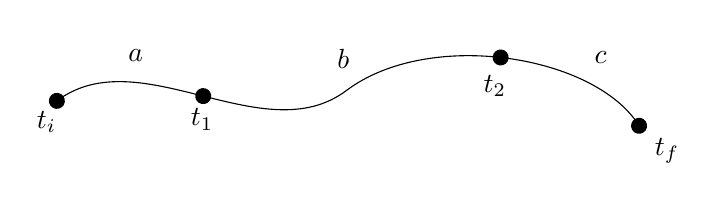
\begin{tikzpicture}[x=0.75pt,y=0.75pt,yscale=-1,xscale=1] 
\draw    (95,115) .. controls (135,85) and (194.5,140) .. (234.5,110) .. controls (274.5,80) and (354.5,93) .. (375.5,127) ;
\draw [shift={(375.5,127)}, rotate = 58.3] [color={rgb, 255:red, 0; green, 0; blue, 0 }  ][fill={rgb, 255:red, 0; green, 0; blue, 0 }  ][line width=0.75]      (0, 0) circle [x radius= 3.35, y radius= 3.35]   ;
\draw [shift={(165.5,112.69)}, rotate = 14.04] [color={rgb, 255:red, 0; green, 0; blue, 0 }  ][fill={rgb, 255:red, 0; green, 0; blue, 0 }  ][line width=0.75]      (0, 0) circle [x radius= 3.35, y radius= 3.35]   ;
\draw [shift={(308.8,94.09)}, rotate = 5.19] [color={rgb, 255:red, 0; green, 0; blue, 0 }  ][fill={rgb, 255:red, 0; green, 0; blue, 0 }  ][line width=0.75]      (0, 0) circle [x radius= 3.35, y radius= 3.35]   ;
\draw [shift={(95,115)}, rotate = 323.13] [color={rgb, 255:red, 0; green, 0; blue, 0 }  ][fill={rgb, 255:red, 0; green, 0; blue, 0 }  ][line width=0.75]      (0, 0) circle [x radius= 3.35, y radius= 3.35]   ;
\draw (90,125) node    {$t_{i}$};
\draw (165,124) node    {$t_{1}$};
\draw (306,108) node    {$t_{2}$};
\draw (389,139) node    {$t_{f}$};
\draw (133,93) node    {$a$};
\draw (233,95) node    {$b$};
\draw (357,94) node    {$c$};
\end{tikzpicture}
\end{figure}
%
\noindent When we consider $t_2<t_1$ the final result is
\[\bra{x_f,t_f}\hat O_1(\hat x(t_1)) O_2(\hat x(t_2))\ket{x_i,t_i}\]
therefore eq.~\eqref{eqn:correlations-path-int} has been proved. Using eq.~\eqref{eqn:correlations-path-int} we can compute matrix element of time ordering products using path integrals. 

\section{The Continuum Limit and Non-Commutativity}
\textsf{Skinner~\cite{Skinner:2018aa} sec. 3.2}\\

Let's go back to an issue we considered in the introduction of the path integral. Now we analyze what happens if the paths we consider are not only the one someone expects, i.e. consider the case where paths are in general not differentiable. The non-commutativity of operators
\begin{equation}\label{eqn:non-comm-PI}
[\hat x(t),\hat p(t)]=i\hbar
\end{equation}
is somehow necessary in order for the path integral to work.  And it is intimately related to the existence of not differentiable path that has to be taken into account in the path integral. We want to show that when we consider all possible path in the computation of the path integral, also non-differentiable path must be taken into account, and this non-differential paths are those to become important when we see non-commutativity of some operators in QM. 

Let's consider only smooth paths, in particular where $\dot x(t)$ exists. Then for $t_-$ slightly smaller than $t$ we have\footnote{We will write $\hat p(x(t))=\dot x(t)$.This is not restrictive, since if we replace $\dot x(t)$ with any other sufficiently regular function the result does not change.}
\begin{align*}
\bra{x_f,t_f}\hat x(t)\,\hat p(t_-)\ket{x_i,t_i}
&=\int_{C_{t_f-t_i}[x_i,x_f]}\mathcal Dx\,x(t)\,\dot x(t_-)e^{\frac i\hbar S[x]}
\end{align*}
Similarly, for $t_+$ slightly greater that $t$
\begin{align*}
\bra{x_f,t_f}\hat p(t_+)\,\hat x(t)\ket{x_i,t_i}
&=\int_{C_{t_f-t_i}[x_i,x_f]}\mathcal Dx\,x(t)\,\dot x(t_+)e^{\frac i\hbar S[x]}
\end{align*}
Since we are considering only smooth path, we have
\begin{align*}
&\lim_{t_\pm\to t}\int_{C_{t_f-t_i}[x_i,x_f]}\mathcal Dx\,x(t)(\dot x(t_-)-\dot x(t_+))e^{\frac i\hbar S[x]}=\\
&\qquad=\int_{C_{t_f-t_i}[x_i,x_f]}\mathcal Dx\,x(t)\p{\lim_{t_\pm\to t}(\dot x(t_-)-\dot x(t_+))}e^{\frac i\hbar S[x]}=0
\end{align*}
and then
\begin{align*}
&\bra{x_f,t_f}\left[\hat x(t)\,\hat p(t)\right]\ket{x_i,t_i}=\\
&\qquad=\lim_{t_\pm\to t}\p{\bra{x_f,t_f}\hat x(t)\,\hat p(t_-)\ket{x_i,t_i}-\bra{x_f,t_f}\hat p(t_+)\,\hat x(t)\ket{x_i,t_i}}=0
\end{align*}
which is clearly in contrast with eq.~\eqref{eqn:non-comm-PI}. The problem is the following: we wrote down the relation between operator formalism and path integral only in the discrete case for $\delta t=T/N=0$ and then we took the continuous limit. We anticipated that this procedure may have some problematic points, that must be considered carefully. 

Let's show this in the simply case of the free particle: $\hat H=\hat p^2/2m$. In order to simplify the notation we set $m=1$. Then the propagator reads
\[K(x_f,t;x_i,0)=\braket{x_f,t}{x_i,0}=\bra{x_f}e^{-i\frac{\hat H}{\hbar}t}\ket{x_i}\]
This satisfies the following relation
\begin{equation}\label{eqn:deriv-prop-free-part}
i\hbar\frac{\partial}{\partial t}K(x_f,t;x_i,0)=\hat HK(x_f,t;x_i,0)
\end{equation}
therefore using eq.~\eqref{eqn:deriv-prop-free-part} and $\hat p=-i\hbar\partial_x$ we can verify the following explicit expression for the propagator\footnote{See \textsf{Rattazzi sec. 1.2.2} for a derivation of this formula.}
\[K(x_f,t;x_i,0)=\frac1{\sqrt{2\pi i\hbar t}}\exp{\frac{i}{2\hbar t}(x_f-x_i)^2}\]
or, with a trivial time translation
\[K(x_f,t_f;x_i,t_i)=\frac 1{\sqrt{2\pi i\hbar (t_f-t_i)}}\exp{\frac{i}{2\hbar}\frac{(x_f-x_i)^2}{t_f-t_i}}\]
Therefore the propagator satisfies following relation
\begin{equation}\label{eqn:derivx-propag-free-part}
-i\hbar \frac{\partial}{\partial x}K(y,t_f;x,t_i)= \frac{x-y}{t_f-t_i}K(y,t_f;x,t_i)=i\hbar \frac{\partial}{\partial y}K(y,t_f;x,t_i)
\end{equation}
The derivative expression of a path can be written as limit of the differential increase rate
\[\dot x(t)=\lim_{\delta t\to0}\frac{x(t+\delta t)-x(t)}{\delta t}\]
If we set $t_+=t+\delta t$ and $t_-=t-\delta t$ we can write, event if $x(t)$ is not differentiable:
\begin{align*}
&\lim_{\delta t\to0}\bra{x_{t_+},{t_+}}\p{\hat x(t)\,\hat p(t_-)-\hat p(t_+)\,\hat x(t)}\ket{x_{t_-},{t_-}}=\\
&\qquad=\lim_{\delta t\to0}\int\de x\bra{x_{t_+},{t_+}}\p{\hat x(t)\,\hat p(t_-)-\hat p(t_+)\,\hat x(t)}\ket x\bra x\ket{x_{t_-},t_-}\\
&\qquad=\lim_{\delta t\to0}\int\de x\braket{x_{t_+},{t_+}}{x,t}x(t)\p{\dot x(t_-)-\dot x(t_+)}\bra{ x,t}\ket{x_{t_-},t_-}\\
&\qquad=\lim_{\delta t\to0}\int\de x\,K(x_{t+\delta t},t+\delta t;x,t)x(t)\p{\frac{x(t)-x(t-\delta t)}{\delta t}-\frac{x(t+\delta t)-x(t)}{\delta t}}K(x,t;x_{t-\delta t},t-\delta t)\\
&\qquad=\lim_{\delta t\to0} \int\de x\,x(t)\,(-i\hbar)\frac\partial{\partial x}\p{K(x_{t+\delta t},t+\delta t;x,t)K(x,t;x_{t-\delta t},t-\delta t)}\\
&\qquad=\lim_{\delta t\to0} \int\de x\,i\hbar K(x_{t+\delta t},t+\delta t;x,t)K(x,t;x_{t-\delta t},t-\delta t)\\
&\qquad=\lim_{\delta t\to0} i\hbar \,K(x_{t+\delta t},t+\delta t;x_{t-\delta t},t-\delta t)
\end{align*}
Where in the second to last step we assumed vanishing boundary terms in the integration by parts. 
So using again composition of paths we obtain
\begin{align*}
\bra{x_f,t_f}\left[\hat x(t)\,\hat p(t)\right]\ket{x_i,t_i}=i\hbar \,K(x_f,t_f;x_i,t_i)
\end{align*}
This is exactly what we desired. It means that all the contributions to the matrix elements of commutators between non-commuting operators is given by non-differentiable paths
\[\lim_{ t_+\to t}\dot x(t_+)\neq\lim_{ t_-\to t}\dot x(t_-)\]
i.e. where velocity shows a discontinuity. If we consider only smooth path, then matrix elements of each commutators would be zero, and this is physically wrong. 









\end{document}